As introduced in Chapter \ref{density_fitting_theory}, density fitting is a method that attempts to reproduce the physical properties of electron density generated by a set of orbitals, using an orbital-free basis set.
\subsection{Metrics} \label{metrics}
To evaluate the various density fitting methods, the following metrics are used:\begin{enumerate}
    \item Mean Absolute Error (MAE) of the Energies (Hartree, External, xc, kinetic)
    \item Mean Absolute Error (MAE) of the of the number of electrons $N = \int \rho(\mathbf{r}) d\mathbf{r}$
    \item The L2 Norm of the difference in densities $\text{L2}[\rho-\rho'] = \sqrt{\int (\rho(\mathbf{r})-\rho'(\mathbf{r}))^2} d\mathbf{r}$
    \item The L1 Norm of the difference in densities $\text{L1}[\rho-\rho'] = \int |\rho(\mathbf{r})-\rho'(\mathbf{r})| d\mathbf{r}$
    \item The Gradient of the total energy at the ground state (Interesting for convergence)
    \item The L1 Norm of negative values in the fitted density $\text{L1}[\rho'] = \int -\rho'(\mathbf{r})\mathbf{1}_{\rho'(\mathbf{r})<0} d\mathbf{r}$
    \item The Hartree energy of the residual density $H_{H}[\rho-\rho'] = \int \int \frac{(\rho(\mathbf{r})-\rho'(\mathbf{r}))(\rho(\mathbf{r'})-\rho'(\mathbf{r'}))}{|\mathbf{r}-\mathbf{r'}|}d\mathbf{r}d\mathbf{r'}$
    \item Standart deviation of the fitted coefficients
\end{enumerate}
\subsection{Density Fitting Methods}

We tested several promising density fitting methods using these metrics. Below, we briefly explain each method’s strengths and the systems they optimize. The detailed derivations are provided in Appendix \ref{appendix
}.

The first few methods are derived from a simple Lagrangian that is minimized without any additional constraints to ensure the conservation of the total integrated density, i.e., the number of electrons.
\subsubsection{Overlap Density fitting}
The simplest density fitting method just minimises the L2 norm of the residual density.
\begin{align} \label{overlap_eq}
        \mathcal{L}(\mathbf{p}) &= \mathbf{p} W \mathbf{p} - 2 \mathbf{p}\bar { L} \bar\Gamma + \bar\Gamma \mathbf{D}\bar\Gamma
\end{align}
As the energies are not directly minimised, they are bound to be very anaccurate.
\subsubsection{Hartree Density fitting}
This method is commonly used in electronic structure calculations to emulate the Hartree energy of the system. It excells in this respect but lacks accuracy in other areas. It minimises the hartree energy of the residual density.
\begin{align}
        \mathcal{L}(\mathbf{p}) &= \mathbf{p} \tilde{W} \mathbf{p} - 2 \mathbf{p}\bar {\tilde L} \bar\Gamma + \bar\Gamma \tilde{\mathbf{D}}\bar\Gamma
\end{align}
\subsubsection{Hartree+External Density Fitting} \label{hartreeexternal}
A simple improvement to the privous method also includes the external energy in the loss function.
\begin{align}\label{true_df}
        \mathcal{L}(\mathbf{p}) &= \mathbf{p} \tilde{W} \mathbf{p} - 2 \mathbf{p}\bar {\tilde L} \bar\Gamma + \bar\Gamma \tilde{\mathbf{D}}\bar\Gamma + (\mathbf{p}\mathbf{v}_{ext}-\bar\Gamma \bar{V}_{ext})^2
\end{align}
But as the external energy enters the equation quadraticly its accuracy tends to be reduced compared to the linear entering hartree energy.
\subsubsection{Hartree+External Density Fitting MOFDFT-Version}
This density fitting method was used in the paper\cite{zhang_m-ofdft_2023} to calculate the labels for the orbital free density. In the paper it was mentioned to minimize the lagrangian above\ref{true_df}, but in reality it minimizes the following lagrangian.
\begin{equation}
    \mathcal{L} &=\left\lVert
    \begin{pmatrix}
    \tilde{W} \\
    v_{ext}^T
    \end{pmatrix}
    \mathbf{p}
    -
    \begin{pmatrix}
    \tilde{L} \bar{\Gamma} \\
    \bar{\Gamma} \bar{V}_{ext}
    \end{pmatrix}
    \right\lVert^2
\end{equation}
Which is similar to the previous method but with the external energy and hartree energy entering the equation in the same way the accuracy is increased.
\subsubsection{Hartree+External Density Fitting with enforced electron number}
This method is identical to Hartree+External density fitting \ref{hartreeexternal} but the number of electrons is enforced by adding a Lagrange multiplier to the loss function.
\begin{align}
    \mathcal{L}(\mathbf{p},\mu) &= \mathbf{p} \tilde{W} \mathbf{p} - 2 \mathbf{p}\bar {\tilde L} \bar\Gamma + (\mathbf{p}\mathbf{v}_{ext}-\bar\Gamma \bar{V}_{ext})^2+\mu(\mathbf{p}\mathbf{w}-\bar\Gamma\bar S)
\end{align}
But this also comes with a decrease in the accuracy of other metrics
\subsubsection{Hartree Density Fitting with enforced electron number and enforced external energy} \label{both_fixed}
To futher utilize lagrange multiplier , we can also enforce the external energy to be exactly reproduced.
\begin{align}
    \mathcal{L}(\mathbf{p},\mu,\nu) &= \mathbf{p} \tilde{W} \mathbf{p} - 2 \mathbf{p}\bar {\tilde L} \bar\Gamma + \nu(\mathbf{p}\mathbf{v}_{ext}-\bar\Gamma \bar{V}_{ext})+\mu(\mathbf{p}\mathbf{w}-\bar\Gamma\bar S)
\end{align}
But this also comes with a decrease in the accuracy of other metrics and it is debatable if it is desirable to enforce a single metric while the reproduced density is of, as this could decrease the stability of the method and lead to unphysical densities.
\subsubsection{Hartree+External Density Fitting MOFDFT-Version with soft enforced electron number}
While not mentioned in the paper\cite{zhang_m-ofdft_2023}, the  corresponding code respory also includes variant of the hartree+external MOFDFT density fitting method with a soft enforced electron number.
\begin{equation}
    \mathcal{L} &=\left\lVert
    \begin{pmatrix}
    \tilde{W} \\
    v_{ext}^T\\
        w^T
    \end{pmatrix}
    \mathbf{p}
    -
    \begin{pmatrix}
    \tilde{L} \bar{\Gamma} \\
    \bar{\Gamma} \bar{V}_{ext}\\
    \bar\Gamma\bar S
    \end{pmatrix}
    \right\lVert^2
\end{equation}
But in praxis reduced the stability of the method while only marginally increasing the accuracy metrics of the total number of electrons.
\subsubsection{Overlap Density fitting with enforced electron number and enforced external energy}
At last we also tested method \ref{both_fixed} while substituding the hartree matrix for the overlap matrix.
\begin{align}
    \mathcal{L}(\mathbf{p},\mu,\nu) &= \mathbf{p} \tilde{W} \mathbf{p} - 2 \mathbf{p}\bar {\tilde L} \bar\Gamma + \nu(\mathbf{p}\mathbf{v}_{ext}-\bar\Gamma \bar{V}_{ext})+\mu(\mathbf{p}\mathbf{w}-\bar\Gamma\bar S)
\end{align}
This leads to a metric which replicates the overall density quite well, but reglects the hartree energy.
\subsection{Results}
We now compare the performance of different density fitting methods using the metrics described above. Ground state densities were calculated for the first 1,000 molecules in the QM9 dataset using Kohn-Sham with the PBE xc-functional and the "6-31G(2df,p)" basis set, then fitted on an even-tempered basis set with $\beta = 2.5$.

The absolute error (AE) of the energies is presented in Figure
\ref{fig:AE_energies}.
\begin{figure}
    \centering
    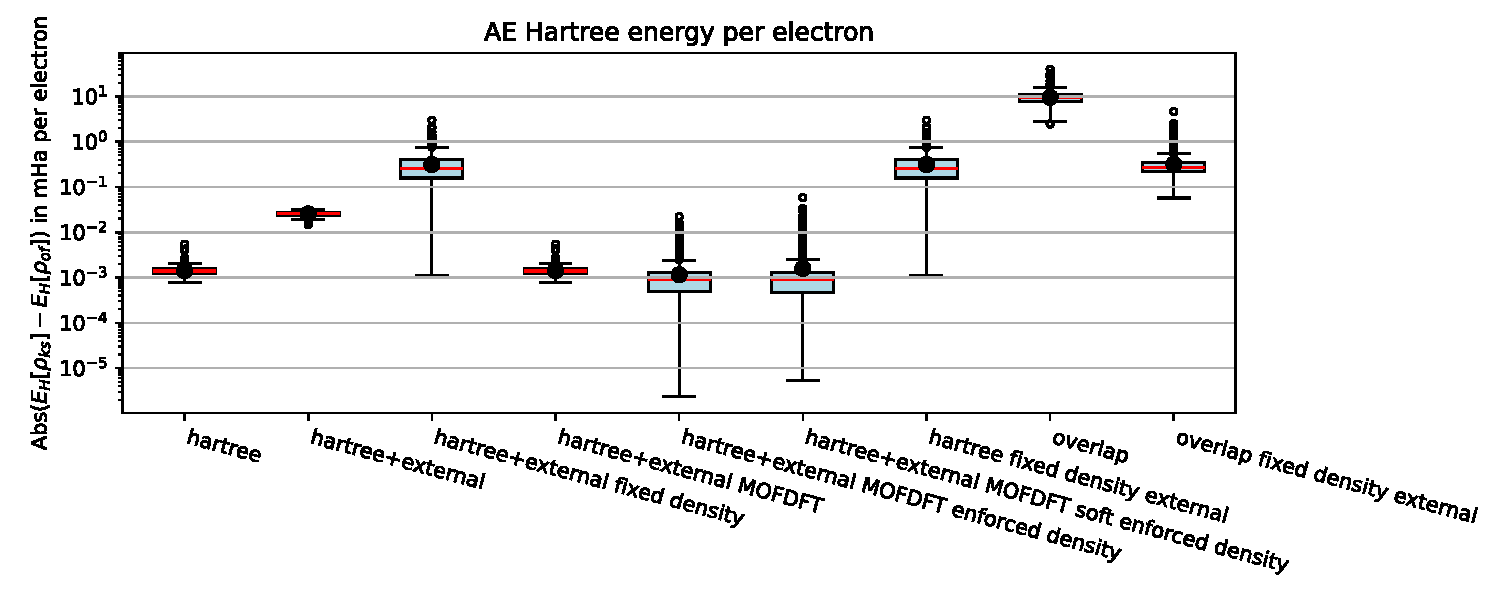
\includegraphics[width=0.9\textwidth]{chapters/results/results_images/AE_hartree_energy_on_even_tempered_2.5_for_different_df_methods}
    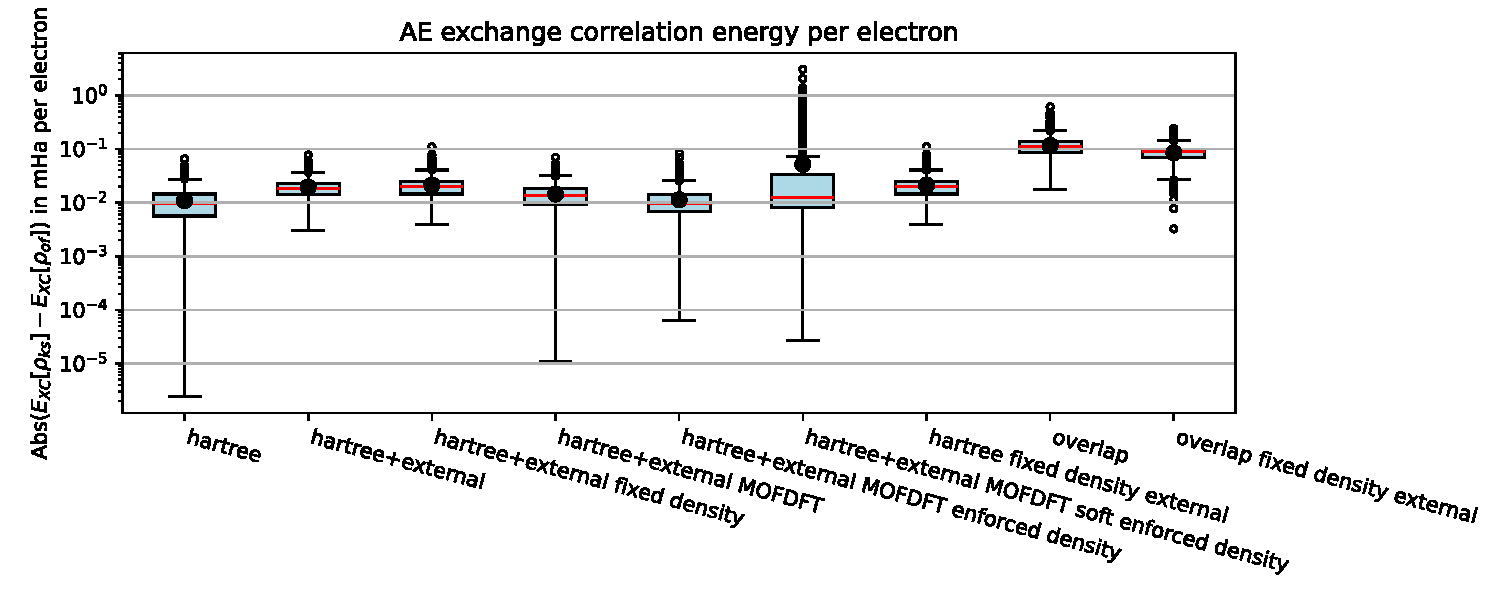
\includegraphics[width=0.9\textwidth]{chapters/results/results_images/AE_xc_energy_on_even_tempered_2.5_for_different_df_methods}
    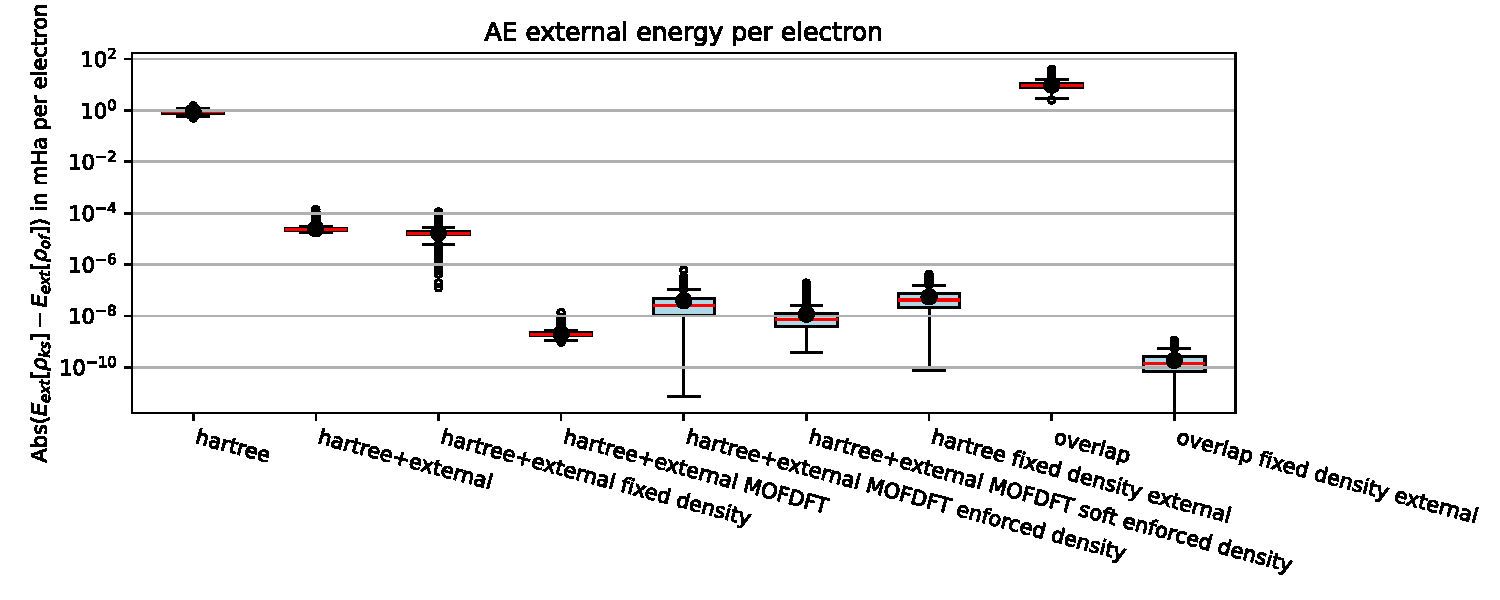
\includegraphics[width=0.9\textwidth]{chapters/results/results_images/AE_ext_energy_on_even_tempered_2.5_for_different_df_methods}
    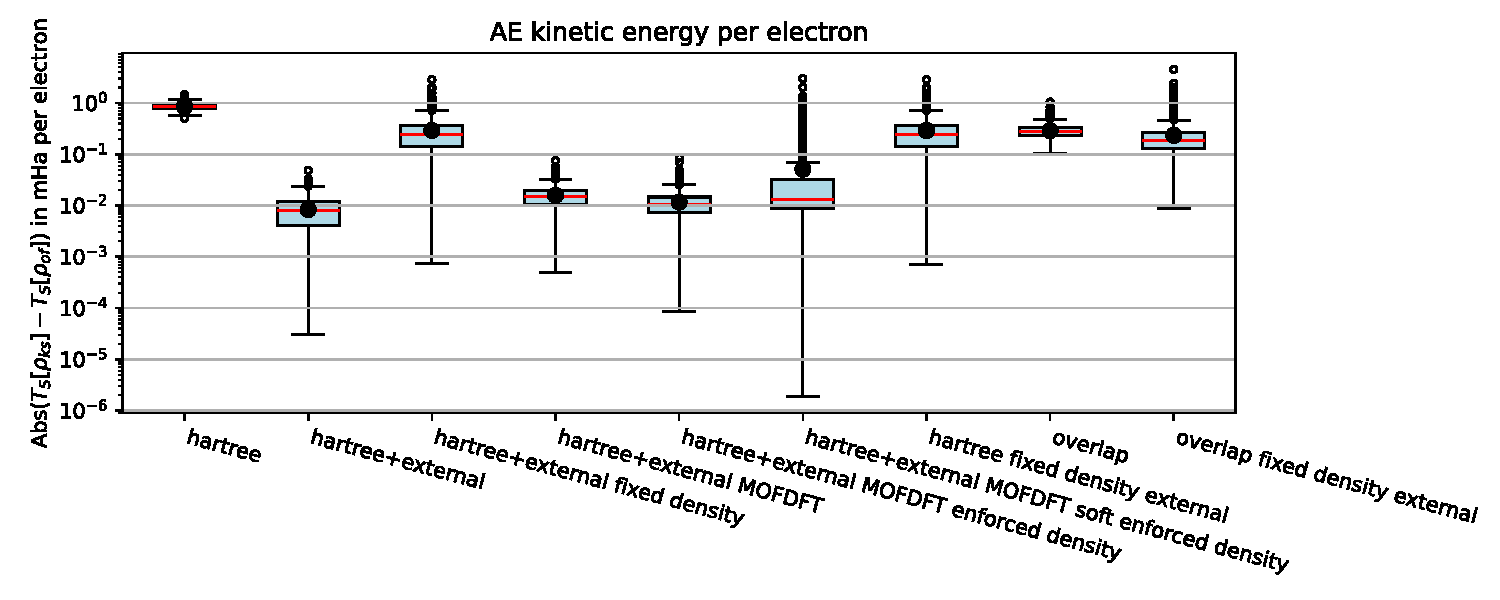
\includegraphics[width=0.9\textwidth]{chapters/results/results_images/AE_kin_energy_on_even_tempered_2.5_for_different_df_methods}
        \caption{Boxplots(\ref{boxplots})) of the AE of Energies per electron for different density fitting methods for the first 1000 molecules in QM9}
    \label{fig:AE_energies}
\end{figure}
We observe that the different density fitting methods generally perform as anticipated. The Hartree, Hartree + external, MOFDFT, and its restricted versions excel at reproducing the total Hartree energy, while the vanilla Hartree + external and its variants appear limited in accuracy. The DF methods that minimize the L2 norm of the residual density perform less effectively, as expected.

For the absolute error (AE) of the exchange-correlation energy, all DF methods perform similarly since none directly optimize this metric, though the overlap methods perform slightly worse. In terms of external energy, the DF methods that directly optimize it produce reliable results. The kinetic energy is best reproduced by the Hartree + external DF method and the various MOFDFT variants.
\begin{figure}
    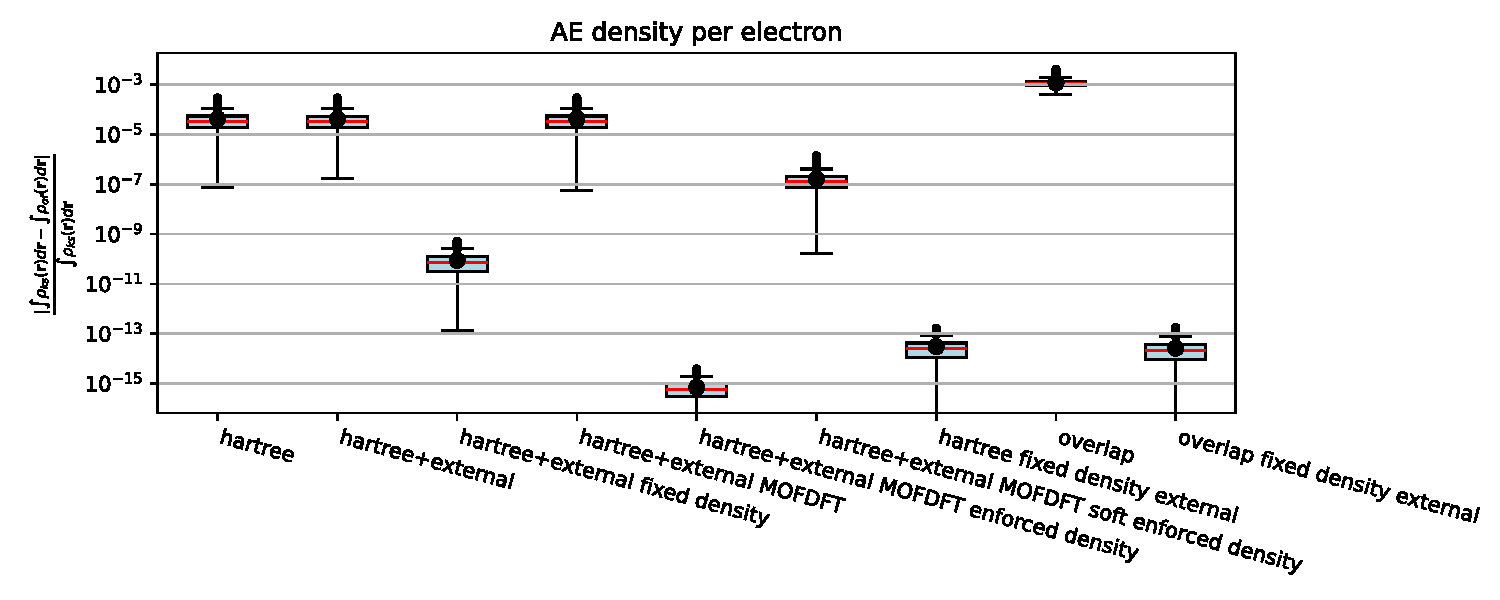
\includegraphics[width=0.9\textwidth]{chapters/results/results_images/AE_density_on_even_tempered_2.5_for_different_df_methods}
    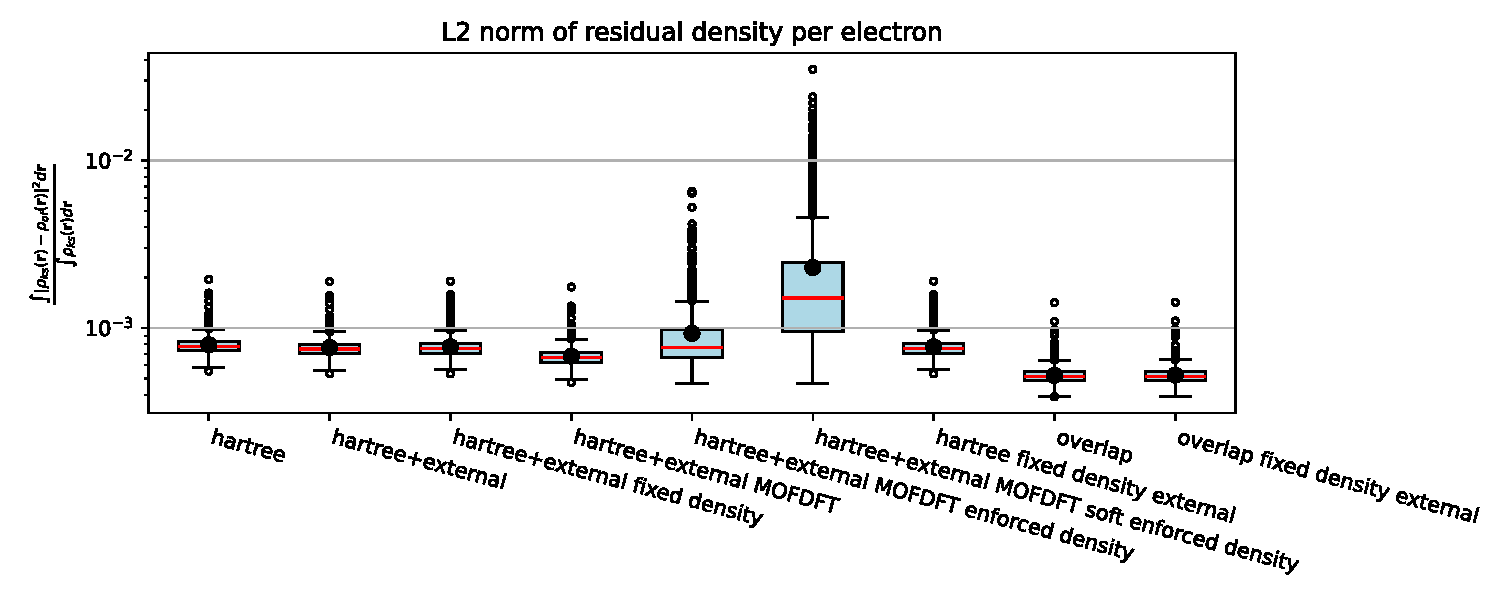
\includegraphics[width=0.9\textwidth]{chapters/results/results_images/L2_residual_densities_on_even_tempered_2.5_for_different_df_methods}
    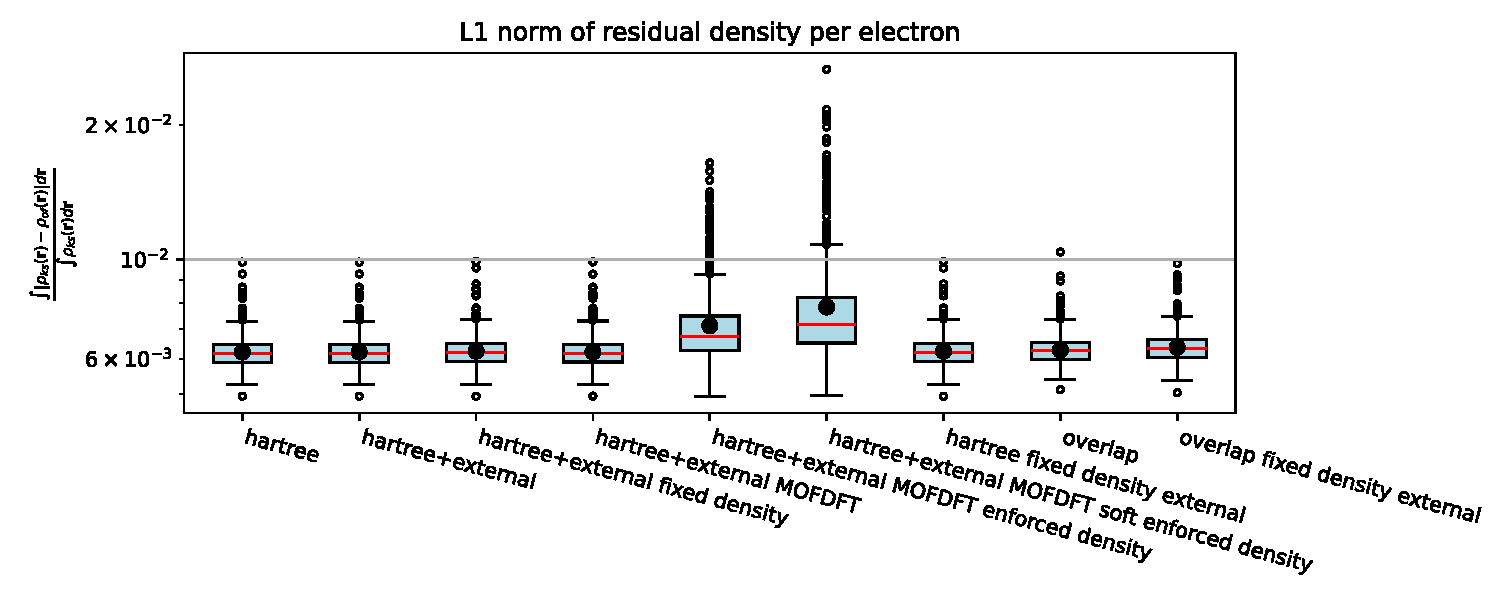
\includegraphics[width=0.9\textwidth]{chapters/results/results_images/L1_residual_densities_on_even_tempered_2.5_for_different_df_methods}
    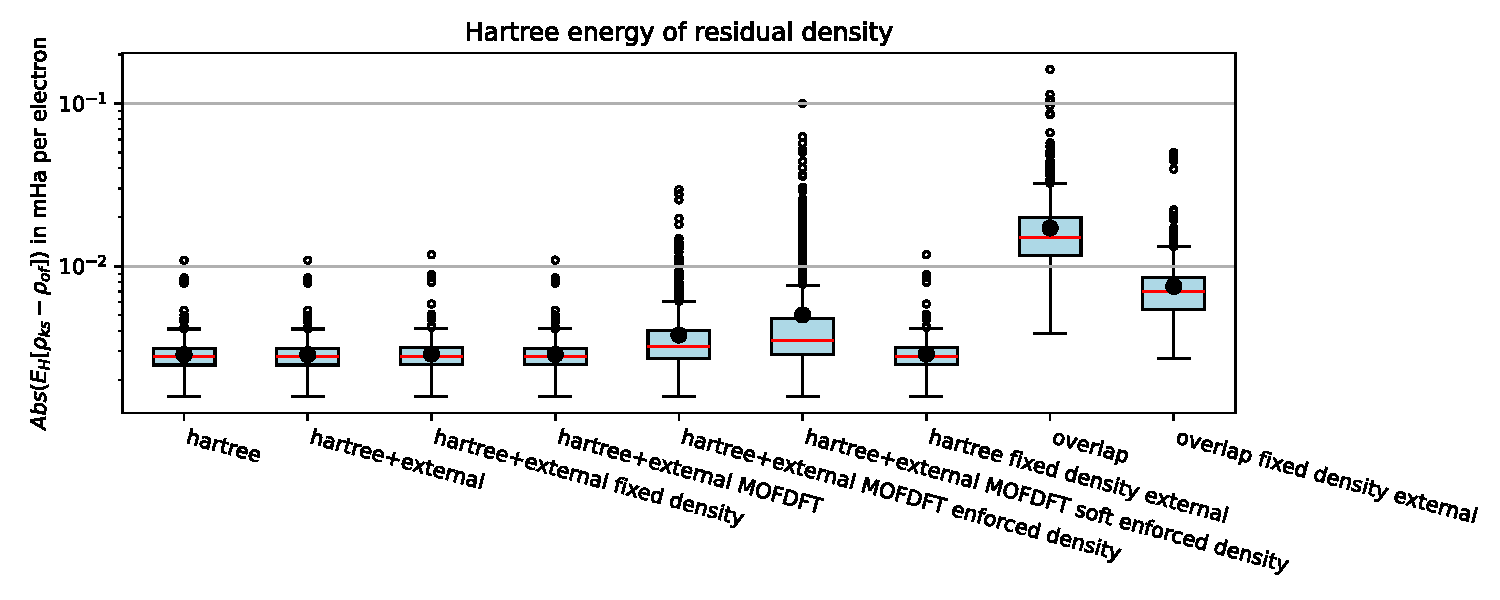
\includegraphics[width=0.9\textwidth]{chapters/results/results_images/L2_residual_hartree_on_even_tempered_2.5_for_different_df_methods}
    \caption{Boxplots(\ref{boxplots})) of the difference in density for different DF - methods}
    \label{fig:Densities_df_methods}
\end{figure}
In figure \ref{fig:Densities_df_methods} we can observe the direct effect of different DF methods on the density. Lets first observe the conservation of electrons. Methods without additional constraints show an absolute error (AE) in the range of 0.01\%–0.1\%, with the overlap method performing the worst. The MOFDFT DF method with a soft constraint improves by two orders of magnitude, and all methods with a hard constraint fulfill this metric up to numerical accuracy. For quality of the fit of the of- densities to the ks densities we have several metrics to observe. The L2 and L1 norm of the residual density are for all DF-methods similary well reproduced with just the soft and hart constraint MOFDFT-versions performing slightly worse, while having a larger spread than the others. Looking the the residual Hartree energy the picture looks similar with the overlap methods performing worse while the other methods perform similarly well.
TODO fix xlabel l2 norm
\begin{figure}
    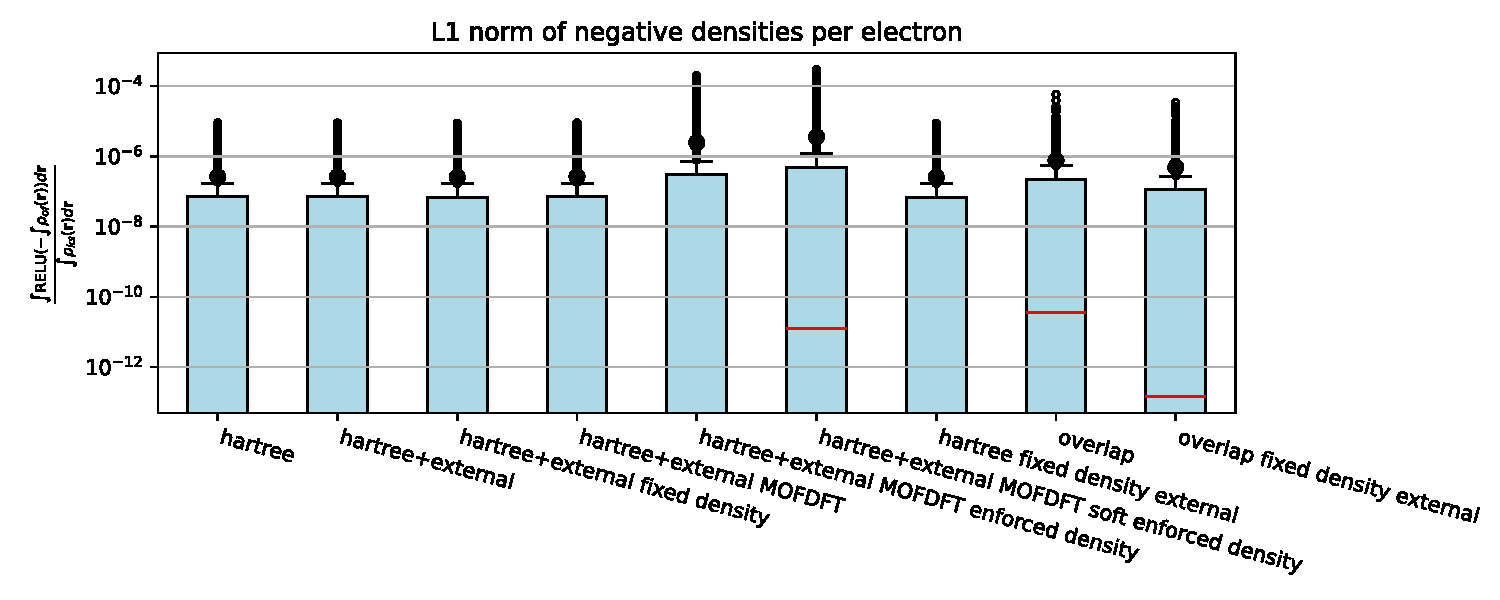
\includegraphics[width=0.9\textwidth]{chapters/results/results_images/L1_negative_densities_on_even_tempered_2.5_for_different_df_methods}
    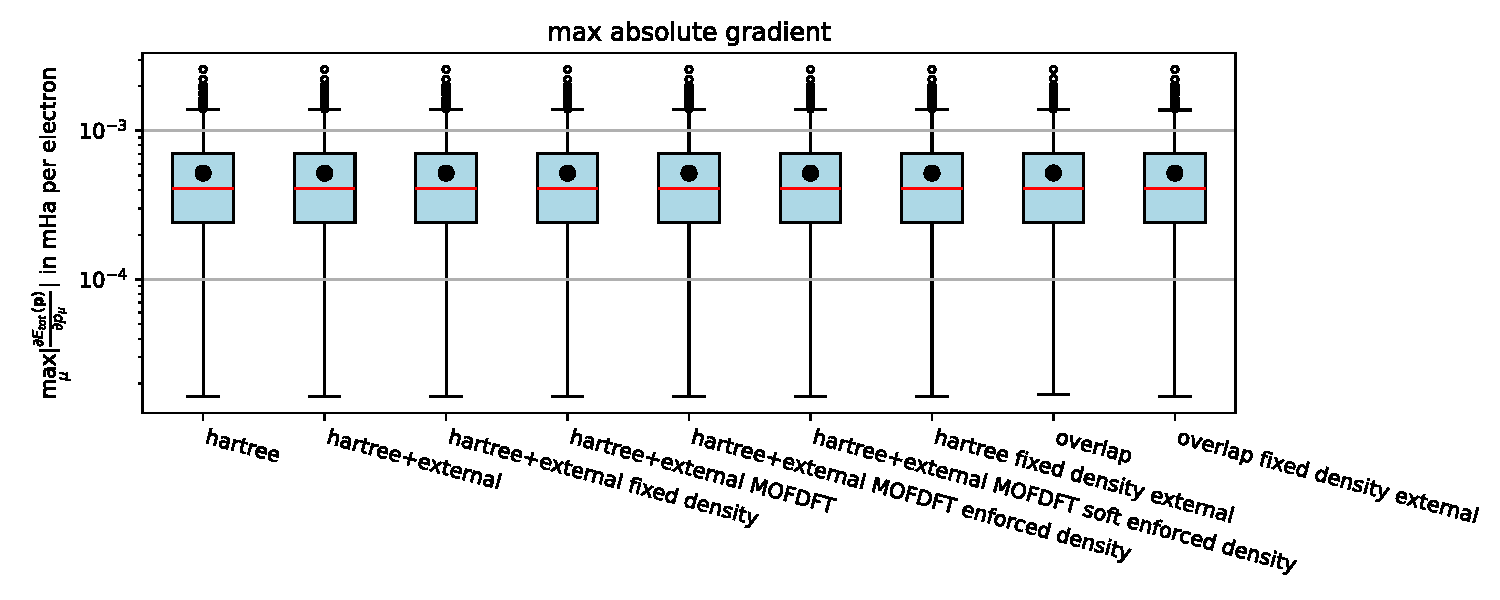
\includegraphics[width=0.9\textwidth]{chapters/results/results_images/max_abs_gradient_on_even_tempered_2.5_for_different_df_methods}
    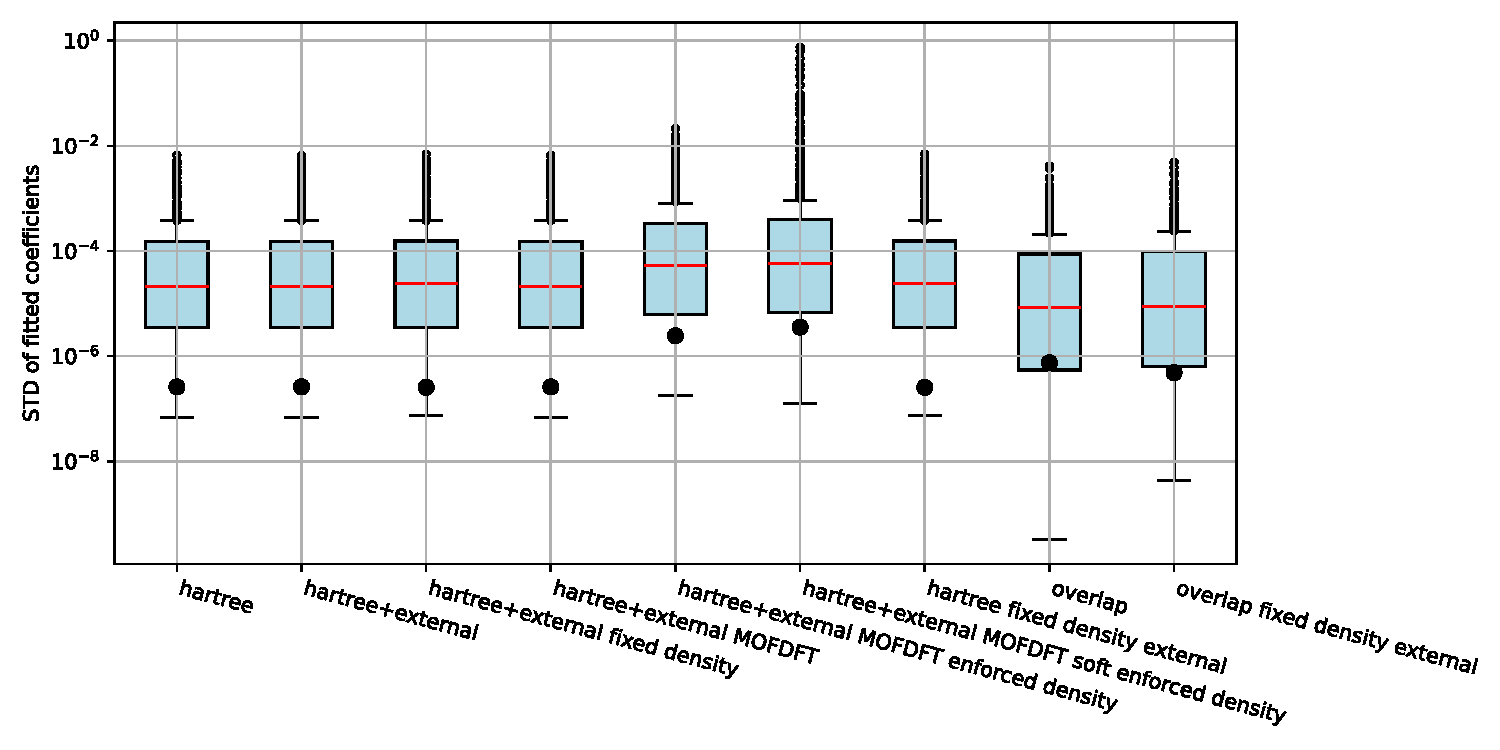
\includegraphics[width=0.9\textwidth]{chapters/results/results_images/var_density_fitting}
    \caption{Boxplots(\ref{boxplots})) of additional metrics which can be used to judge the stability of the DF-methods}
    \label{fig:other_df_metrics}
\end{figure}
There are a few more metric we can take a look at, depicted in figure \ref{fig:other_df_metrics} that can be worth to take a look at. The L1 norm of negative values is something to look out for, as they are unphysical and are not visible in the other metrics. As we can see the negative densities are mostly quite low with only a few outliers for the constraint MOFDFT versions and overlap methods to reach critical values. The gradient of the total energy is calculated using the procedere explained in \ref{labelgen_gradient} and should be zero at the ground state. Because of this the maximum of the gradient is a meainingfull metric for the quality of density fitting. For the tested DF - methods no meaning full difference could be observed between them. At last we are going to take a look at the standart deviation of the fitted coefficients which can be seen a a metric for the stability of the method. Here the individual event aren't the first 1000 molecules of QM9 but instead the individual exponents of the fitted basis set for each atom type as can be seen in \ref{var_coeffs}. Where we can see that the soft constraint MOFDFT versions is performing the worst.
\begin{figure}
    \centering
    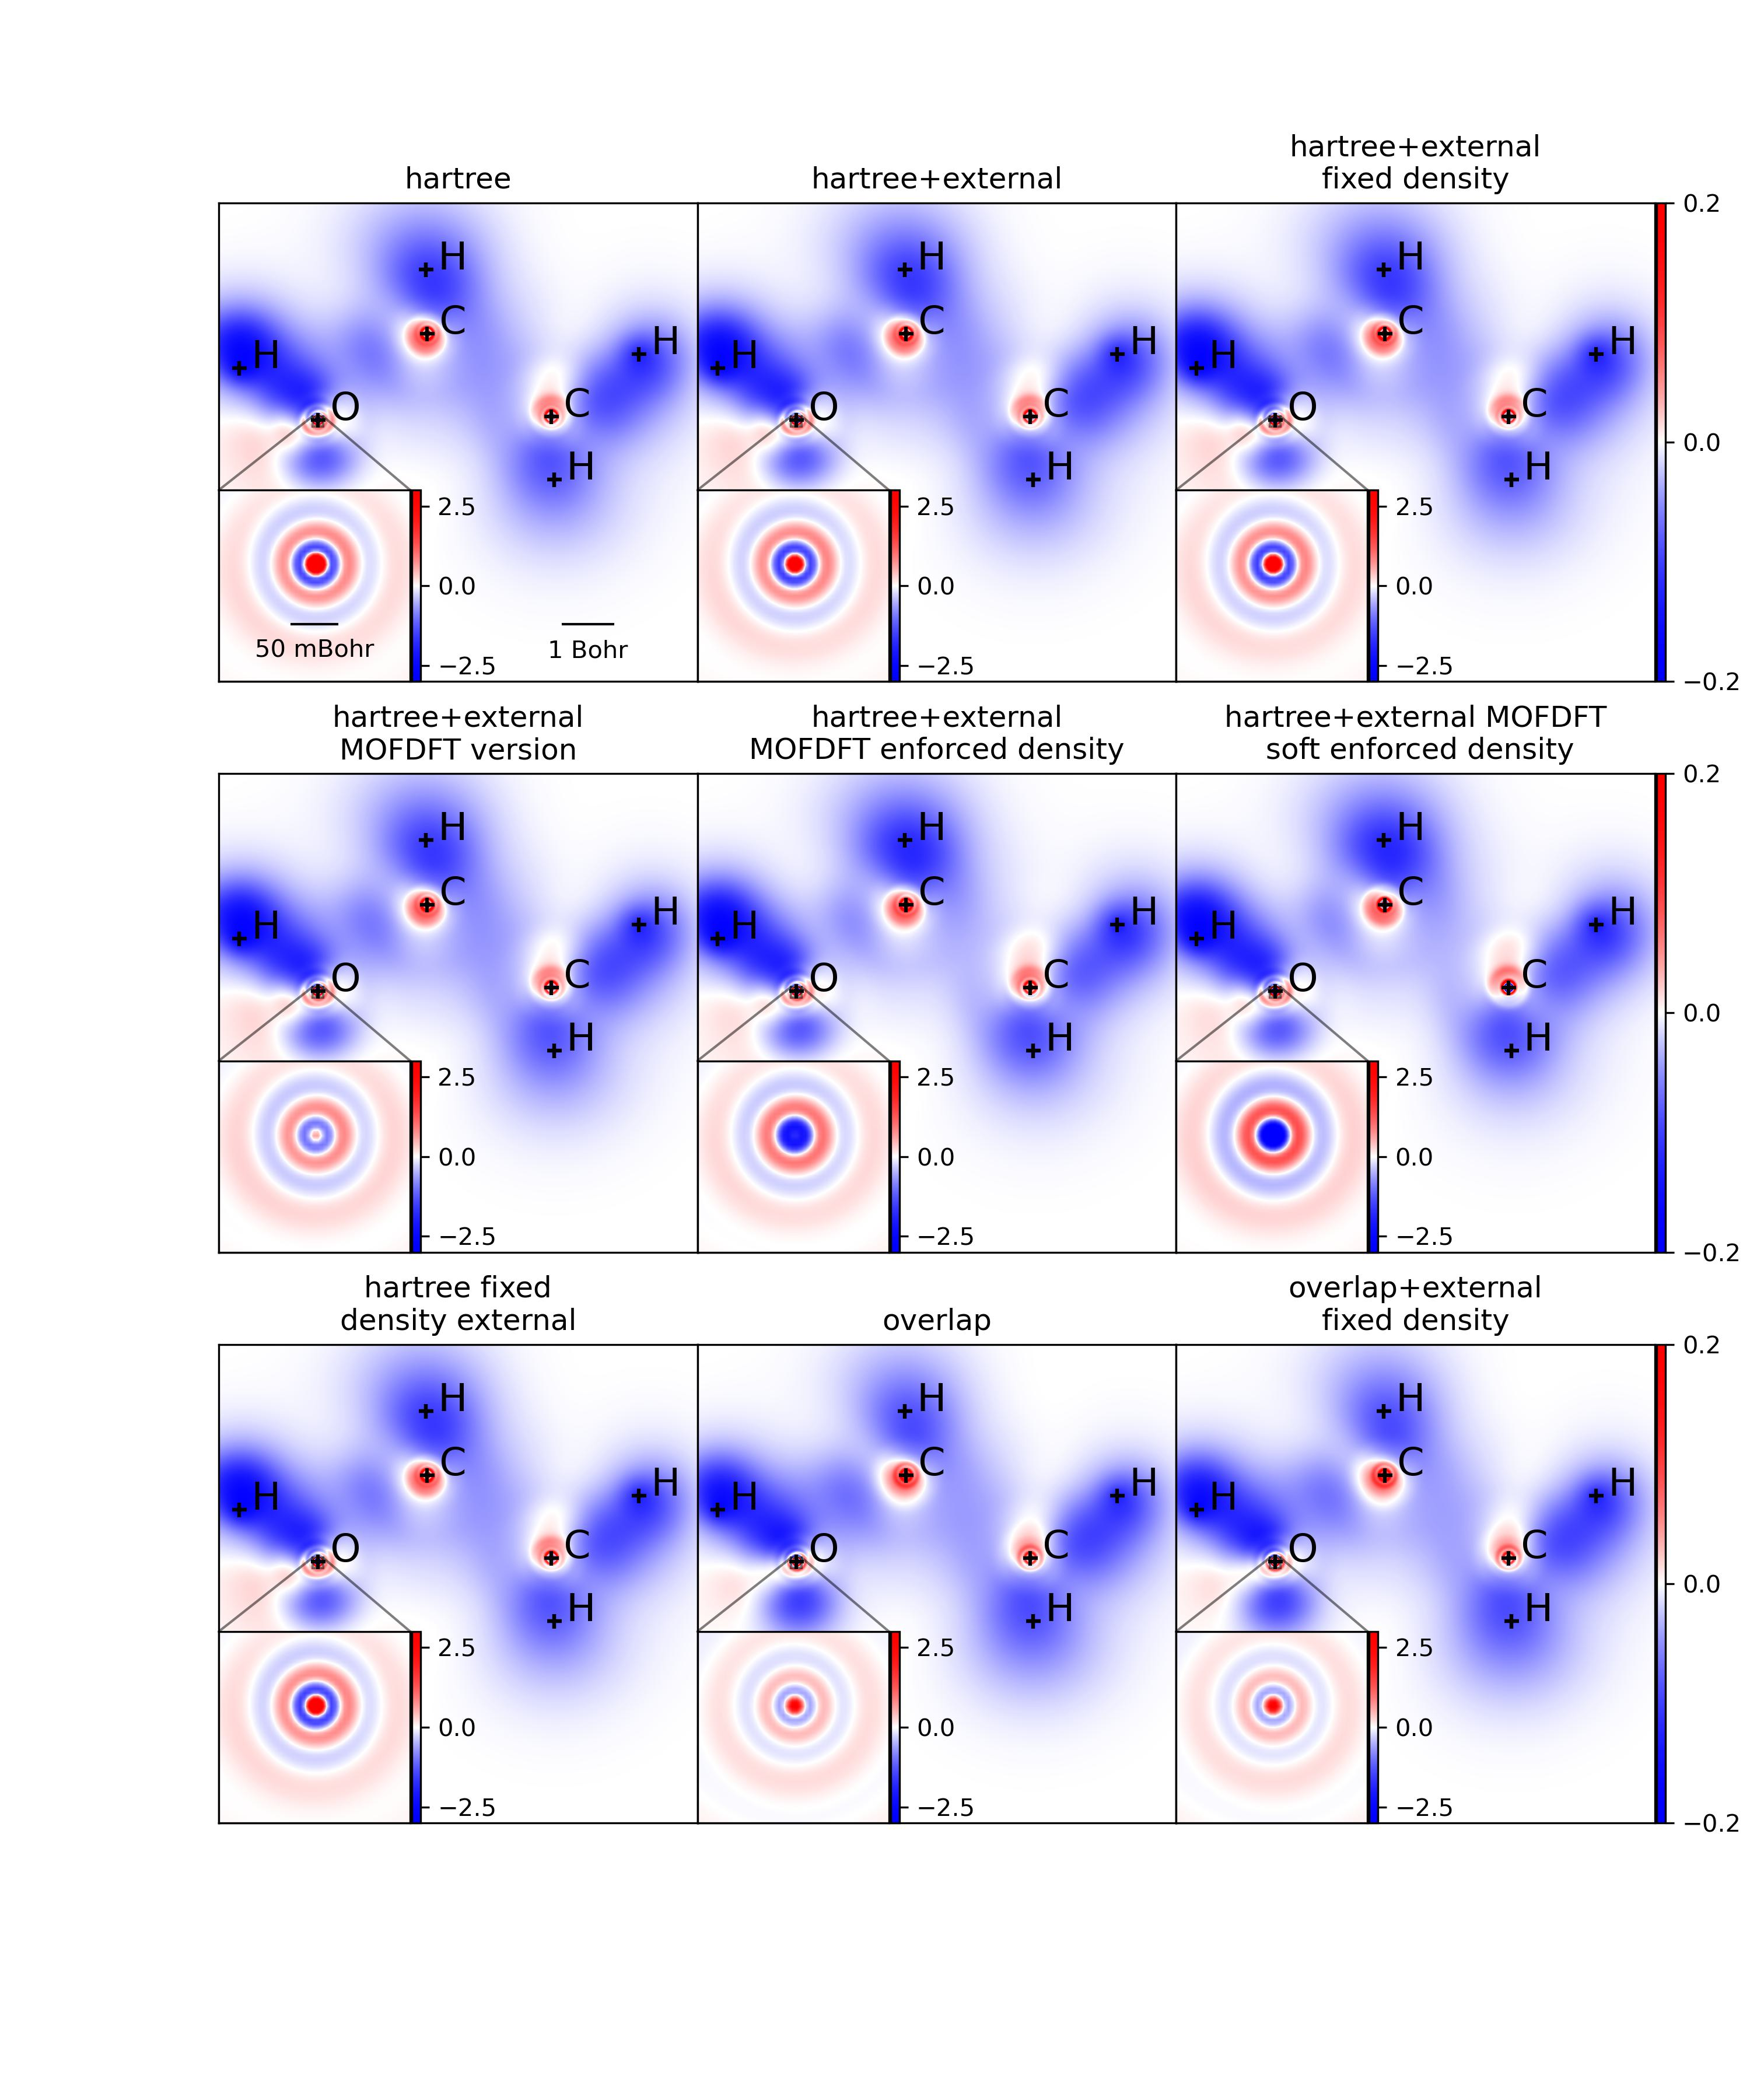
\includegraphics[width=1\textwidth]{chapters/results/results_images/density_fitting_slices_new}
    \caption{A visualisation of the differences in densities between the fitted and the original densities using slices of a Ethanol molecule}
    \label{fig:density_slices_df}
\end{figure}
Another way of judging the quality of a fit is to take a look a t the difference in density directly. In figure \ref{fig:density_slices_df} we plotted the difference in density for in the form of 2d slices which are laid through the symmetry axis of an Ethanol molecule. As most of the density of an molecule is located around the atomic nuclei, also the biggest density errors are exspected to be there. Here we can also see that the differences in density between the different methods are mostly very suttle and can hardly seen with the bare eye. The lowest visible difference can be seen for the overlap methods. This is to be exspected as these methods aim to provide the closed fit at any point in space, which is exactly what is visualized in the plots.
\subsection{Conclusion}
In summary, we found that the distinct density fitting methods fulfill different roles. The methods based on minimizing the L2 norm of the residual density perform the best for optimizing just this metric. However, for the reproducibility of the individual energies, it is necessary to use a method based on minimizing the Hartree energy of the residual density. We found that out of the unrestricted methods, the Hartree+external MOFDFT version performed the best all around, producing reliably good energies, as well as good and stable densities, while not producing too many negative densities. Its only caveat is that it doesn't exactly conserve the number of electrons. This drawback is fixed by the use of constrained methods, which perform a minimization while fixing the correct number of electrons, at the cost of slightly worse energies and densities. The hard constrained version of Hartree+external MOFDFT performs very well at this job, reproducing almost the same energies as its unrestricted version with just slightly worse and more unstable densities, a higher amount of negative densities, and higher variance of the coefficients. If stability and conservation of the number of electrons are of concern, then the method "Hartree fixed densities and external energy" is a good choice, as it performs very well all around with just slightly worse energies than the other methods.







